\section{Introdução} \label{section: Introducao}
\setstretch{1.15}
Nos dias de hoje, a escolha entre sistemas operativos \textit{open source} e proprietários é uma decisão crucial para as empresas. Esta escolha envolve uma série de considerações, desde o objetivo do nosso sistema ou software até às implicações legais do licenciamento e às preocupações com a segurança e estabilidade.
\par \vspace{6pt}
Neste trabalho vamos explorar estes tópicos fazendo a comparação entre sistemas operativos \textit{open source} e proprietários e apresentando as suas características, destacando também a importância do \textit{kernel} e as suas responsabilidades na operação de um sistema operativo.
\par \vspace{6pt}
Analisando o caso específico do GNU/Linux, vamos falar da sua história e da importância de ambos o \textit{kernel} Linux e do projeto GNU na sua criação. Iremos ainda falar da sua presença em diferentes ambientes.
\par \vspace{6pt}
Discutimos as complexidades do licenciamento \textit{open source}, examinando as implicações legais e práticas para empresas que optem por utilizar software de \textit{open source}.
\par \vspace{6pt}
Investigaremos a segurança dos sistemas operativos \textit{open source}, analizando quais os principais riscos no seu uso. 
\par \vspace{6pt}
Por fim, analisaremos o processo de utilização de software \textit{open source} em ambientes empresariais, explorando os desafios e benefícios associados à adoção deste modelo de software.
\vspace{10pt}
\begin{figure}[H]
  \centering
  % width=\textwidth para imagem da largura do texto
  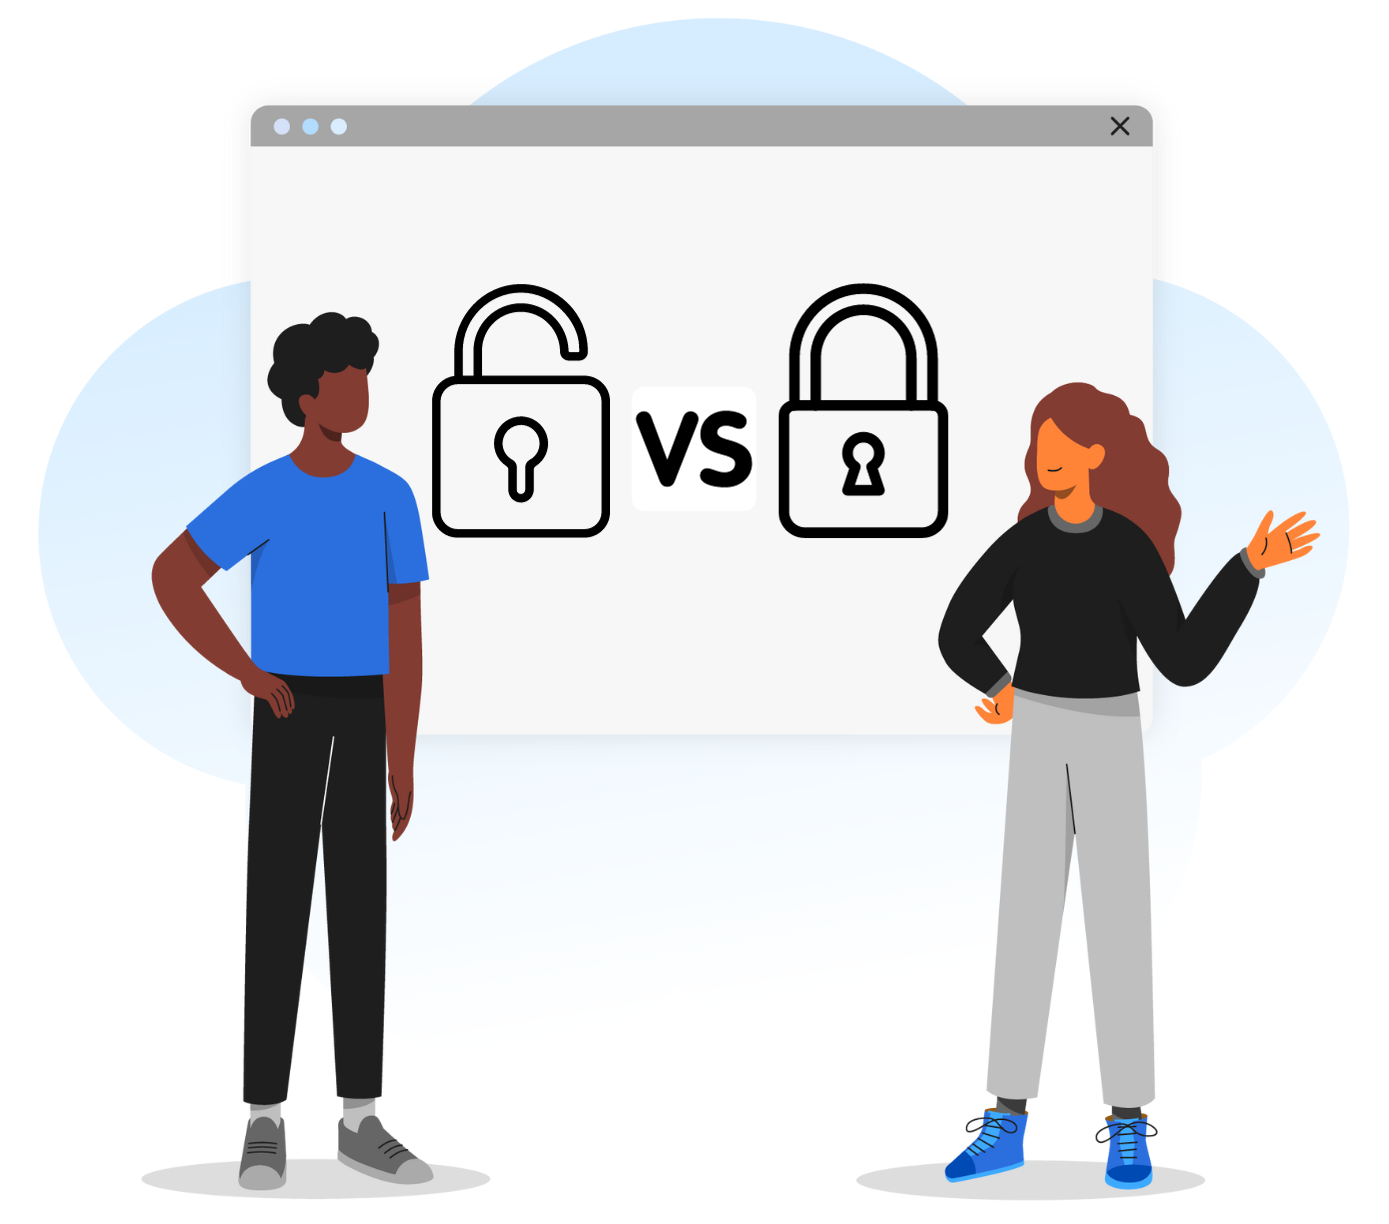
\includegraphics[scale=0.30]{Figures/0. General/open_vs_closed.png}
  \caption{\textit{open source} contra \textit{closed source}}
  \label{Open source vs. closed source}
\end{figure}